\chapter{\label{ch:lit_review} Literature Review}

This literature review provides a comprehensive exploration of the integration of Augmented Reality (AR) with mobile robotics, focusing on its applications in Human-Robot Interaction (HRI). The review is structured to cover several key areas that are crucial to the development of an AR framework for a 4WD robotic car. Here's an overview of what readers can expect to find in this literature review:

\begin{figure}[ht]
    \centering
    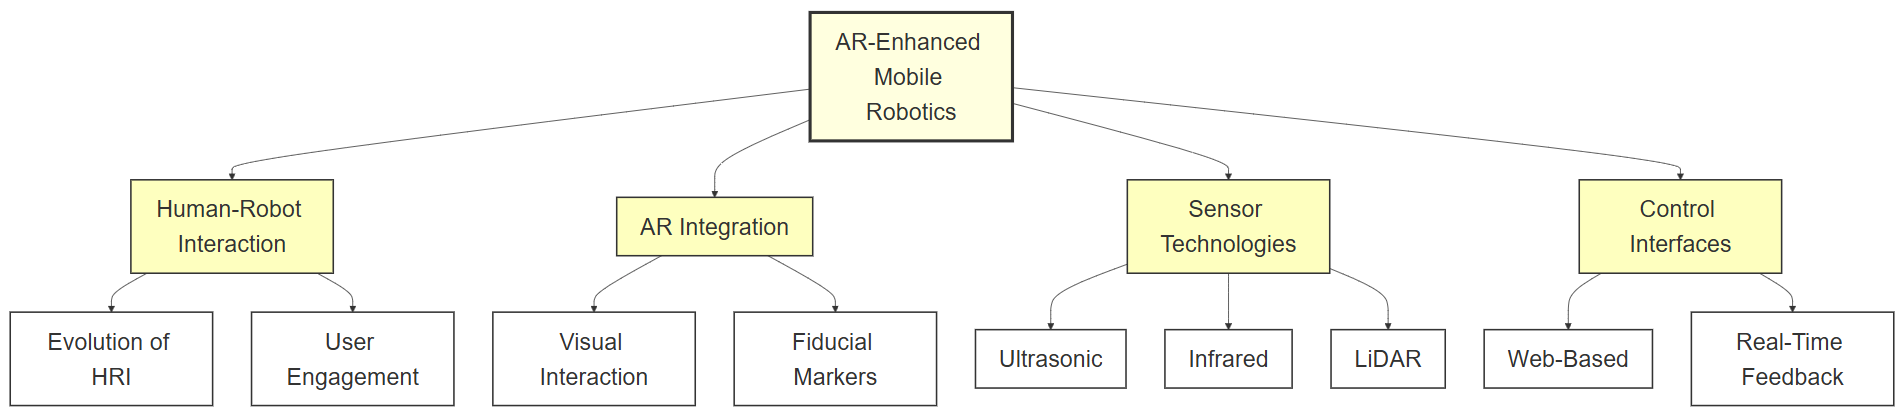
\includegraphics[width=1\textwidth]{ch2/figs/lit_overview.png}
    \caption{Overview of the structure of the literature review}
    \label{fig:Lit_overview}
\end{figure}

\section{Introduction to Human-Robot Interaction (HRI) and Augmented Reality (AR)}

Human-Robot Interaction (HRI) has seen substantial growth in both research and industrial applications, particularly with the advent of collaborative robots (cobots) that work alongside humans in dynamic environments. These robots, unlike their predecessors, are designed to safely interact with humans in shared workspaces, marking a significant shift in industrial automation. 

According to \cite{Hentout2019}, HRI evolved from isolated robot systems in manufacturing to collaborative systems where robots assist humans in complex tasks. This shift is largely due to advancements in sensing, control, and human-machine interface technologies that allow robots to perceive their environment and interact intelligently.

\begin{figure}[ht]
    \centering
    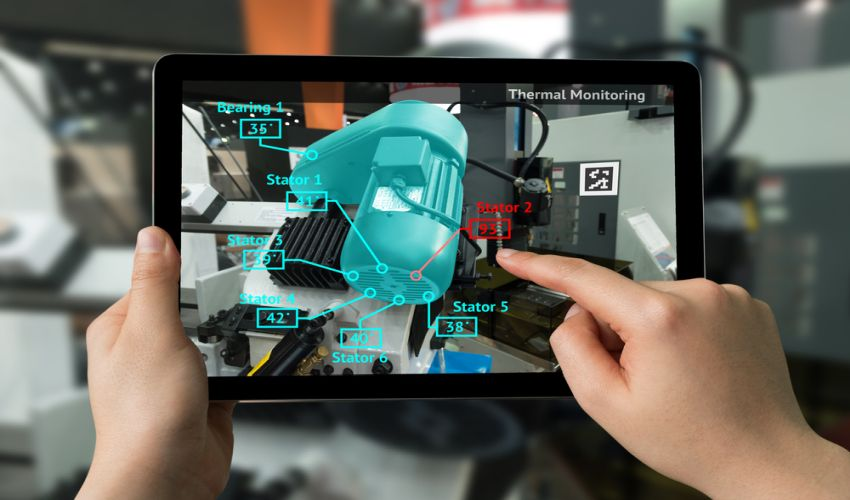
\includegraphics[width=0.8\textwidth]{ch2/figs/image_overlay.png}
    \caption{Screen Display of work environment with AR additions}
    \label{fig:AR_work_overlay}
\end{figure}

Augmented Reality (AR) has emerged as a powerful tool in enhancing HRI by providing a more intuitive and efficient way for humans to interact with robots. AR serves as a bridge that overlays digital information onto the physical environment, enabling users to better understand the robot’s actions and the task at hand \cite{Suzuki2022}. 

\subsection{Virtual Reality in Human-Robot Interaction: A Comparison with Augmented Reality}

Virtual Reality (VR) and Augmented Reality (AR) have both played significant roles in advancing Human-Robot Interaction (HRI). However, their applications and interaction paradigms differ significantly. Understanding these differences is essential when analyzing how each technology enhances the interaction between humans and robots.

VR offers a fully immersive experience where users interact with robots in a completely simulated world. This makes it particularly effective for applications such as robotic training, simulation, and remote teleoperation. For instance, VR is widely used for training operators and robots in new tasks in a risk-free virtual environment \cite{Coronado2023}. By immersing the user in a fully virtual environment, VR allows for complex robot interactions, including simulated task execution and environment navigation, which is especially useful in fields such as disaster response, industrial automation, and surgical simulations \cite{Gul2022}.

AR, on the other hand, overlays digital information onto the real world, making it more suitable for real-time, operational tasks involving physical robots. AR enables users to view critical information such as navigational data, sensor outputs, or planned robot trajectories without losing connection to their real-world environment \cite{García2019}. This makes AR ideal for applications where humans and robots share the same workspace, such as collaborative manufacturing, logistics, and maintenance tasks.

While both technologies are beneficial, this literature review will primarily focus on Augmented Reality due to its practical applications in human-robot collaboration. 

\subsection{Augmented Reality as a Tool in HRI}

AR enhances communication between humans and robots by offering real-time visualizations and feedback, thus improving situational awareness and reducing errors in task execution. Suzuki et al. \cite{Suzuki2022} propose a taxonomy of AR-enhanced HRI, highlighting the key areas where AR plays a role, such as task guidance, real-time interaction, and environment mapping. In particular, AR’s ability to provide visual feedback significantly enhances the user experience by making robot operations more transparent and reducing cognitive load.

Moreover, AR facilitates dynamic task interaction by enabling users to provide real-time instructions to the robot. This is particularly beneficial in industrial applications where task conditions change frequently. AR not only improves task accuracy but also contributes to a more efficient workflow, as robots can quickly adjust their behavior based on user commands and visual markers such as ArUco codes \cite{Suzuki2022}.

AR's applications in HRI span various industries, from manufacturing to healthcare. In manufacturing, AR has been utilized to guide robot operations through real-time visual overlays, improving precision and safety in tasks that require close human-robot collaboration \cite{Hentout2019}. Similarly, in healthcare, AR assists medical robots in performing delicate procedures by providing real-time feedback and guidance, enhancing both safety and operational efficiency \cite{Suzuki2022}. 

\section{Mobile Robotics and AR Integration}

The integration of Augmented Reality (AR) in mobile robotics has transformed how robots communicate their intentions and interact with their environment. AR not only enhances human-robot collaboration but also provides an intuitive interface for users to understand robot behavior in dynamic and complex environments. Several key studies have explored the use of AR to improve robot navigation, task execution, and real-time interaction between humans and robots.

\subsection{AR as a Communication Tool in Mobile Robotics}

One of the primary challenges in human-robot interaction is communicating the robot’s intended actions to human operators. Spatial Augmented Reality (SAR) has proven to be an effective method for achieving this. In the study by Green et al. \cite{Green2019}, SAR is used to project information about the robot’s intended movement directly onto the physical environment. This method allows users to better anticipate and respond to the robot’s actions, reducing uncertainty and enhancing collaboration. Michalos et al. \cite{Michalos2022} demonstrated the application of AR in industrial settings, where visual feedback aids in task coordination between humans and robots, leading to improved task accuracy and faster response times.

Additionally, Coovert et al. \cite{Coovert2014} explored how spatial AR techniques can improve communication between robots and humans. In their experiment, a robot used visual projections of arrows and simplified maps on the floor to indicate its short-, mid-, and long-term movement intentions. The study found that participants were able to predict the robot’s movements with high confidence when the robot projected its intended path. This is especially useful in environments where humans and robots share a workspace, such as hospitals, museums, and factories.

\begin{figure}[ht]
    \centering
    \begin{subfigure}[b]{0.4\textwidth}
        \centering
        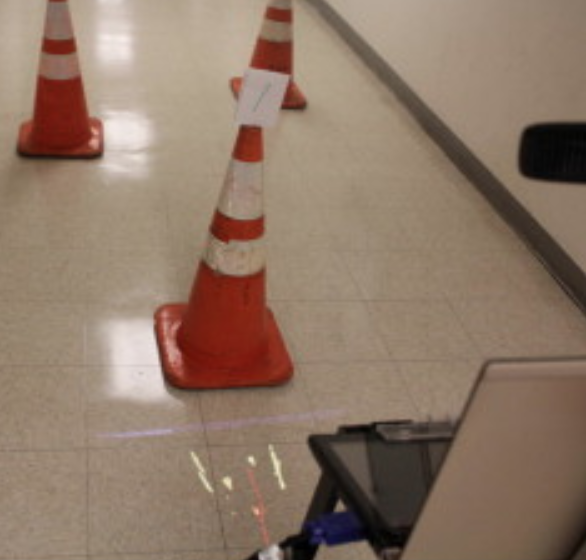
\includegraphics[width=\textwidth]{ch2/figs/robot_nav2.png}
        \caption{Robot estimating its intended movement. \cite{Coovert2014}.}
        \label{fig:estimating_path}
    \end{subfigure}
    \hspace{0.05\textwidth} % Adjust the space between the images as needed
    \begin{subfigure}[b]{0.32\textwidth}
        \centering
        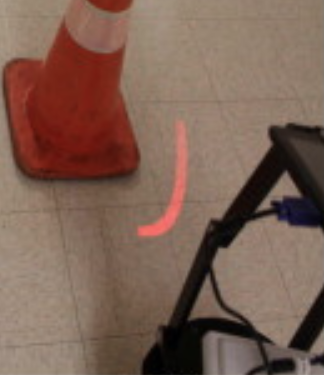
\includegraphics[width=\textwidth]{ch2/figs/robot_nav_1.png}
        \caption{Robot estimating its intended movement using AR arrows \cite{Coovert2014}.}
        \label{fig:intended_path}
    \end{subfigure}
\end{figure}



\subsection{Multimodal AR Interfaces for Human-Robot Interaction}

In addition to visual feedback, multimodal interfaces that combine AR with other modalities, such as voice or gesture recognition, have further improved human-robot interaction. Green et al. \cite{Green2019} developed a multimodal AR interface for mobile robots, allowing users to interact with the robot through visual overlays, voice commands, and gesture-based inputs. This interface improved the efficiency and accuracy of task execution in collaborative environments. The study demonstrated that multimodal AR interfaces allow for more flexible and adaptive human-robot communication, making the interaction process more intuitive and reducing cognitive load on the user.

\subsection{Applications of AR in Mobile Robotics}

AR’s integration into mobile robotics is particularly useful in environments that require constant adaptation, such as manufacturing or logistics. Michalos et al. \cite{Michalos2022} applied AR in human-robot cooperation in industrial settings, where robots must adapt to rapidly changing conditions. AR provided real-time feedback to users, helping them coordinate with robots for tasks such as assembly or quality control. Moreover, AR visualizations helped robots better navigate dynamic environments, improving both safety and efficiency.

Furthermore, AR’s ability to create real-time visual overlays in the robot’s workspace has significant implications for task planning and execution. In particular, SAR-based interfaces allow users to visually instruct robots by marking control zones or highlighting obstacles, which the robot then interprets for navigation and task completion \cite{Coovert2014}.

\subsection{Challenges and Future Directions}

While AR’s role in mobile robotics has demonstrated significant potential, challenges remain in real-time processing, accurate object recognition, and user feedback latency. As Michalos et al. \cite{Michalos2022} noted, the integration of AR into robotic systems requires further advancements in sensor technology and computational power to ensure real-time responsiveness in dynamic environments. Future research will likely focus on improving AR’s scalability in complex settings, refining multimodal interfaces, and enhancing the autonomy of mobile robots to handle more sophisticated tasks.



\section{Fiducial Marker Systems in HRI}

Augmented Reality (AR) is increasingly used in robotics to facilitate various types of Human-Robot Interactions (HRI). While multiple interaction modalities have been discussed, the remainder of this literature review will focus specifically on visual and marker-based interactions. Below is a list of the different types of interactions possible with AR:

\begin{itemize}
    \item \textbf{Visual Interaction}: AR overlays visual cues such as control zones, instructions, and real-time status feedback, enhancing human comprehension of the robot's operational environment.
    \item \textbf{Gesture-Based Interaction}: Human gestures can be interpreted by robots through AR-enhanced vision systems, reducing reliance on manual interfaces.
    \item \textbf{Speech and Command Interaction}: AR, combined with voice recognition, allows users to issue commands to robots with visual aids providing additional context.
    \item \textbf{Fiducial Marker-Based Interaction}: Fiducial markers such as ArUco or AprilTags provide robots with a way to interpret their environment, helping with localization, navigation, and object detection.
\end{itemize}

\subsection{Fiducial Marker Systems Overview}

In AR-enhanced HRI, fiducial marker systems are essential for real-time contextual interactions. These systems use visually distinct markers that robots detect through cameras. The most commonly used marker systems include ARToolKit, AprilTags, and ArUco markers, each with unique characteristics suited to various applications.
\begin{figure}[ht]
    \centering
    \begin{subfigure}[b]{0.25\textwidth}
        \centering
        
\includegraphics[width=\textwidth]{ch1/figs/ARToolkit.jpg}
        \caption{ARToolKit}
        \label{fig:artoolkit}
    \end{subfigure}
    \hfill
    \begin{subfigure}[b]{0.25\textwidth}
        \centering
        
\includegraphics[width=\textwidth]{ch1/figs/AprilTag.png}
        \caption{AprilTags}
        \label{fig:apriltags}
    \end{subfigure}
    \hfill
    \begin{subfigure}[b]{0.25\textwidth}
        \centering
        
\includegraphics[width=\textwidth]{ch1/figs/ArUco.png}
        \caption{ArUco markers}
        \label{fig:aruco}
    \end{subfigure}
    \caption{Visual comparison of different marker systems}
    \label{fig:markers}
\end{figure}

\textbf{ARToolKit} is one of the earliest fiducial marker systems developed for augmented reality applications. It was widely adopted in early AR systems due to its simplicity and moderate computational requirements. In HRI, ARToolKit has been used in early experiments involving robot navigation and control. However, its robustness is limited compared to more modern systems, and it struggles under challenging lighting conditions \cite{Suzuki2022}.

\textbf{AprilTags} are an improvement over ARToolKit, offering significantly higher robustness and detection accuracy. As \cite{Daponte2020} highlights, AprilTags are designed to provide accurate detection even in adverse environments with variable lighting and occlusion. AprilTags have been extensively used in industrial applications where precise localization is critical, such as warehouse automation and autonomous guided vehicles (AGVs). The system is computationally heavier than ARToolKit but provides superior reliability, making it suitable for applications that demand accuracy over speed \cite{Filus2023}.

\textbf{ArUco markers} are designed with computational efficiency in mind, offering high detection speed without sacrificing much in terms of accuracy. This makes them ideal for real-time applications, particularly in mobile robotics where swift responses are critical. \cite{Husar2022} notes that ArUco markers have been used in various applications including navigation and task execution in dynamic environments such as warehouses. Their simplicity and widespread software support make them a popular choice for developers working on real-time robotic systems.

\begin{table}[h]
\centering
\caption{Comparison of Fiducial Marker Systems}
\resizebox{\textwidth}{!}{
\begin{tabular}{|p{3.1cm}|p{2.1cm}|p{2.1cm}|p{3.2cm}|p{4.5cm}|}
\hline
\textbf{Marker System} & \textbf{Robustness} & \textbf{Detection Accuracy} & \textbf{Computational Efficiency} & \textbf{Applications} \\
\hline
ARToolKit     & Moderate    & Good      & Moderate      & Early AR applications \\\hline
AprilTags     & High        & Excellent & Moderate-High & Robotics \\\hline
ArUco Markers & High        & Good      & High          & Real-time robot navigation \\
\hline
\end{tabular}
}
\end{table}


\subsection{Choosing the Best Marker System for the Project}

Given the requirements of the project, which involve real-time processing, dynamic navigation, and user interaction, ArUco markers are the most suitable choice. As \cite{Filus2023} demonstrates, ArUco markers provide a good balance between computational efficiency and detection accuracy, making them ideal for mobile robotic systems that require fast decision-making. Additionally, the ease of integration with commonly used robotics software such as ROS (Robot Operating System) further justifies their selection for this project.

\subsection{Visual Interaction in AR-Enhanced HRI}

Visual interaction is one of the most common and effective forms of interaction in Augmented Reality (AR)-enhanced Human-Robot Interaction (HRI). It enables users to interact with robots by visualizing contextual information directly within their physical environment. This can include task instructions, control zones, and real-time feedback on the robot's status and performance.

In AR-enhanced visual interaction, the robot's actions and intentions are augmented with overlays that help the human user make informed decisions during interaction. \cite{Suzuki2022} provides a comprehensive overview of how visual interaction enhances HRI by improving situational awareness and reducing the complexity of controlling robotic systems. This is especially useful in industrial applications, where workers interact with robots to execute precise tasks, such as assembly and quality control.

\subsubsection{Applications of Visual Interaction}

Visual interaction in AR has broad applicability across various fields, with significant benefits in improving task accuracy, communication, and overall efficiency. Some notable applications include:
\begin{itemize}
    \item \textbf{Manufacturing and Assembly}: In industries such as automotive and aerospace, visual interaction is used to overlay task instructions on the assembly line, helping workers follow complex procedures. This reduces human error and increases productivity by providing step-by-step visual guidance \cite{Daponte2020}.
    \item \textbf{Healthcare}: In robotic surgery and rehabilitation, visual interaction allows surgeons and therapists to see real-time data overlaid on patients, enhancing precision and safety. AR enhances the accuracy of procedures by showing virtual boundaries and guidelines, ensuring that robots move correctly within the workspace \cite{Husar2022}.
    \item \textbf{Warehouse and Logistics}: In logistics and warehouse management, AR systems provide real-time visual cues to workers handling robotic systems for item sorting, picking, and delivery. \cite{Husar2022} explores the use of AR to improve warehouse efficiency by overlaying instructions on specific zones, helping workers interact more intuitively with robotic arms and autonomous guided vehicles (AGVs).
\end{itemize}

\subsubsection{Visual Feedback and Real-Time Interaction}

One of the most significant advantages of AR-enhanced visual interaction is the provision of real-time feedback, which facilitates more intuitive robot control. \cite{Filus2023} investigates the real-time testing of vision-based systems in AGVs using ArUco markers and AR visualizations. Their research highlights how visual feedback improves decision-making in dynamic environments, helping robots navigate autonomously with greater efficiency.

Visual feedback can take various forms:
\begin{itemize}
    \item \textbf{Control Zones}: Specific areas within the robot's environment are highlighted using AR, guiding the robot's actions and helping the user visualize where the robot can move or interact with objects.
    \item \textbf{Status Updates}: Information such as battery levels, current tasks, or environmental hazards can be projected onto the robot’s workspace, allowing users to quickly assess and adjust the robot’s behavior as needed.
    \item \textbf{Error Detection}: AR systems can visually highlight potential errors in the robot's movements, such as collisions, off-course navigation or wheel slipping, enabling quick corrective actions.
\end{itemize}


Suzuki et al. \cite{Suzuki2022} emphasizes that visual interaction not only enhances HRI but also promotes collaboration between human operators and robots by reducing cognitive load. By providing real-time visual cues, AR improves situational awareness and makes controlling robots more intuitive, particularly in environments where precision is critical.

However, there are certain limitations. \cite{Daponte2020} discusses the challenges of accurately overlaying visual data in real-time, particularly in environments with inconsistent lighting, reflections, or occlusions. Additionally, the processing demands of rendering real-time visualizations may limit the performance of systems with constrained computational resources.

\section{AR's Role in Improving User Engagement}

Augmented Reality (AR) has significantly enhanced user engagement with robotic systems, particularly in Automated Guided Vehicles (AGVs). By providing intuitive visual feedback and real-time streaming data, AR improves both the psychological and practical interaction between humans and AGVs. The combination of augmented reality and robotics has been a topic of significant research interest, as AR makes robots more intuitive to control and increases user trust in automated systems.

\subsection{Enhancing User Engagement through Real-Time Feedback and Visualization}

One of the key strengths of AR is its ability to provide real-time feedback and visualizations, allowing users to intuitively understand the robot’s actions and status. AR-infused streaming technology improves human-robot collaboration by projecting real-time data, control zones, and navigation paths onto the robot's environment \cite{Fu2023}. This continuous stream of real-time data reduces cognitive load, enabling users to anticipate and control AGV movements more effectively in dynamic environments. Such real-time visualization allows users to engage more deeply with robotic systems, increasing their confidence in controlling AGVs.

In particular, \cite{Fu2023} explore how AR is utilized across different robotic applications, including medical, industrial, and social robotics. For AGVs, they highlight AR's capability to enhance human-robot collaboration by improving real-time task allocation and decision-making processes. The visual feedback offered by AR systems reduces the need for constant manual adjustments, thereby increasing operator efficiency \cite{Fu2023}.

In industrial scenarios, \cite{Makhataeva2020} emphasize the role of AR in improving user engagement through its intuitive interfaces. They note that AR helps operators visualize tasks more clearly, thus reducing the learning curve for new users while providing advanced feedback for experienced operators. This is important in environments where quick decisions are necessary \cite{Makhataeva2020}.

\subsection{Psychological and Practical Benefits}

The psychological impact of AR on user engagement is considerable. Real-time visualizations, such as path projections or task instructions, create a more predictable and transparent interaction between humans and robots. Users become more confident when they can clearly see an AGV's next move, which reduces uncertainty about the robot's behavior and enhances user trust. This \textbf{increased predictability} improves user satisfaction and promotes wider adoption of AR-enabled robotic systems \cite{Coovert2014}.

AR also offers practical benefits in rehabilitation settings, where users can engage with robotic systems in therapy. As Makhataeva \cite{Makhataeva2020} points out, AR interfaces allow users to interact with AGVs or rehabilitation robots in a natural way, improving patient recovery outcomes. The immersive nature of AR encourages patient involvement, which is crucial in therapeutic contexts \cite{Makhataeva2020}.

\section{Web-Based Control Interfaces}
Having a functional robot is all well and good but if the robot has an unpleasant or inefficient interface then it ruins the whole user experience. This section will detail different methods of implementing web-based control interfaces, focusing on real-time communication, user interaction, and video streaming. 

\subsection{Webserver Framework Options}

\textbf{Flask} is a lightweight Python web framework known for its simplicity and flexibility\cite{moraneus2024}. It is particularly well-suited for the rapid development of web-based control interfaces. Flask is easy to set up and use, making it ideal for prototyping and small to medium-sized applications. It integrates well with Python libraries commonly used in robotics. However, for real-time features, additional libraries may be required, and its performance can be a concern for large-scale applications.

\textbf{Node.js} is a JavaScript runtime built on Chrome’s V8 engine, recognized for its event-driven, non-blocking I/O model. Its asynchronous nature makes it highly suitable for real-time applications \cite{asiandigitalhub2023}. Node.js also benefits from a large ecosystem of packages and libraries and is capable of efficiently handling many simultaneous connections. However, it may require more setup compared to Flask, and its callback-based programming can be complex for beginners.

\textbf{WebSocket integration} is essential for real-time control and data streaming, providing low-latency, bidirectional communication over a single TCP connection \cite{websockets}. This is particularly advantageous when sending control commands and receiving video streams. WebSockets can be integrated with both Flask and Node.js, though careful implementation is required to handle issues such as connection drops and reconnections, and additional security measures may be necessary.

\textbf{Apache and Nginx} are traditional web servers that are robust, highly scalable, and performant, making them popular choices in production environments. They offer extensive documentation and strong security features. However, they may be more complex to set up and configure, and can be overkill for smaller projects or embedded systems like Raspberry Pi \cite{jankov2019}. They are typically used in conjunction with application servers rather than for standalone dynamic content.

Flask or Node.js, combined with WebSocket integration, would likely be the most suitable choices due to their ease of use and real-time capabilities. For this project Flask will be implemented due to its ease of understanding for a beginner.

\subsection{Security and User Experience}

While security is a crucial aspect of any robotic system, especially those controlled through web-based interfaces, it's important to note that for the scope of my project, I've chosen not to delve deeply into privacy and security concerns. This decision allows me to focus more intensively on the core functionality and user experience aspects of the system.

In a real-world application, however, it would be critical to implement robust security measures. These would typically include encryption protocols like TLS (Transport Layer Security) to protect the integrity and confidentiality of data exchanged between the robot and the user interface. Additionally, strong authentication mechanisms would be necessary to prevent unauthorized access to the robot's controls.

\section{Sensor Technologies in Human-Robot Interaction}

When discussing the AR technology, it's difficult to do so without making mention of sensors, sensors allow machines to interact with their environments. Sensors are to machines what eyes and ears are to humans. This section serves as a review for the applicable sensors relevant to this project which is designing a AR framework for a 4WD robotic car.

\subsection{Ultrasonic Sensors} 
Ultrasonic sensors are a common choice in mobile robotics due to their effectiveness in obstacle avoidance and distance measurement. These sensors emit ultrasonic waves and measure the time it takes for the waves to reflect back from an object, allowing the robot to calculate the distance from obstacles \cite{maupin2023ultrasonic}. This capability provides spatial awareness that is critical for safe navigation. Below is a basic diagram showcasing the operation of an HC-SR04 Infrared Sensor.

\begin{figure}[ht]
    \centering
    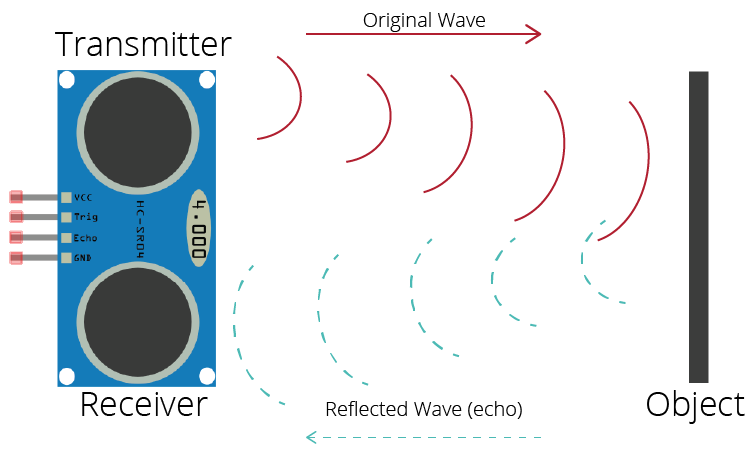
\includegraphics[width=0.53\textwidth]{ch2/figs/ultrasonic_sensor.png} % Change the path if the image is located elsewhere
    \caption{Operation of an Ultrasonic Sensor {\cite{randomnerd2021ultrasonic}}}
    \label{fig:ultrasonic_sensor}
\end{figure}

\noindent
Below is a comparison of some common ultrasonic sensors used in mobile robotics.

\begin{table}[ht]
\centering
\caption{Comparison of Ultrasonic Sensors}
\begin{tabularx}{\textwidth}{|c|c|X|c|c|c|}
\hline
\textbf{Model} & \textbf{Range (cm)} & \textbf{Operating Voltage (V)} & \textbf{Accuracy} & \textbf{Field of View} & \textbf{Size (mm)} \\ \hline
HC-SR04 & 2-400 & 5 & ±0.3 cm & 15 degrees & 45 x 20 x 15 \\ \hline
Maxbotix MB1000 & 20-645 & 2.5-5.5 & ±1\% & 42 degrees & 22 x 20 x 16 \\ \hline
Parallax PING))) & 3-300 & 5 & ±0.5 cm & 20 degrees & 22 x 46 x 16 \\ \hline
\end{tabularx}
\label{tab:ultrasonic_comparison}
\end{table}

Ultrasonic sensors are advantageous because of their simplicity, affordability, and ease of integration. For this project, they could provide an excellent mechanism for detecting nearby obstacles, which is essential for navigation in dynamic environments. Some key properties of ultrasonic sensors include:

\begin{itemize}
    \item \textbf{Wide Range of Detection}: As seen in the table, ultrasonic sensors like the HC-SR04 and Maxbotix MB1000 can detect objects at distances ranging from a few centimeters to several meters. This is beneficial for both short-range and long-range obstacle avoidance.
    \item \textbf{Accuracy and Precision}: Depending on the model, ultrasonic sensors offer good accuracy for distance measurements. For example, the Maxbotix MB1000 boasts an accuracy of ±1\%, helping ensure that the robot reacts promptly and effectively to its surroundings.
    \item \textbf{Field of View (FoV)}: The field of view differs between sensors, affecting the robot's perception. A larger FoV allows the robot to detect obstacles from a wider angle, but may result in less precise focus on individual objects.
\end{itemize}

Integrating ultrasonic sensors with augmented reality (AR) offers the possibility of visualizing sensor data in real time. For example, AR can highlight areas where the robot detects obstacles, providing the operator with enhanced spatial awareness, preventing collisions, and improving task efficiency. Additionally, real-time data streaming through a visual interface allows for immediate adjustments to the robot's behavior based on sensor readings.

\subsection{Infrared Sensors} 

Infrared (IR) sensors are commonly used in mobile robotics for tasks such as proximity detection, line-following, and object avoidance. These sensors emit infrared light and detect the reflection from nearby objects, making them effective for short-range detection in controlled environments \cite{benet2002infrared}.

While standard IR sensors, such as the basic proximity IR sensors, serve well in obstacle avoidance and object detection, they have limitations in terms of range, field of view, and accuracy. These standard sensors perform well in specific lighting conditions but struggle in environments with significant ambient light interference \cite{rhydo2024}.


The \textbf{Dagu Infrared Compound Eye} shares basic functionality with standard IR sensors but offers significant enhancements. Unlike single-point IR sensors, the Dagu sensor features a compound array of multiple infrared detectors, allowing for a much wider field of view and multi-directional sensing. This enables the robot to detect objects from multiple angles, enhancing spatial awareness and enabling more complex navigation and object tracking tasks \cite{rhydo2024}.

Integrating the \textbf{Dagu Infrared Compound Eye} into this project would extend the robot's capabilities by improving its obstacle detection, particularly in dynamic and complex environments. The sensor’s wide field of view, combined with real-time AR feedback, could provide users with a more intuitive control system and greater situational awareness, thereby improving human-robot interaction (HRI). Moreover, the sensor could aid in tasks requiring precise spatial awareness, such as navigating around obstacles or detecting specific objects \cite{benet2002infrared}.

\begin{table}[ht]
\centering
\caption{Specifications of the Dagu Infrared Compound Eye}
\begin{tabular}{|c|c|}
\hline
\textbf{Specification} & \textbf{Value} \\ \hline
Number of Detectors & 4 infrared sensors \\ \hline
Detection Range & 200mm \\ \hline
Operating Voltage & 5V \\ \hline
Power Consumption & 10 mA \\ \hline
\end{tabular}
\label{tab:dagu_infrared}
\end{table}


Additionally, this sensor could provide valuable data that could be visualized for the user through augmented reality (AR), enabling a more interactive and user-friendly experience.

\subsection{LiDAR Sensors} LiDAR (Light Detection and Ranging) is an essential technology for mobile robotics that uses laser light to measure distances and create 3D maps of environments. By utilizing LiDAR sensors, mobile robots can detect obstacles, map their surroundings, and navigate autonomously \cite{yang2022lidar}.

\begin{figure}[hb]
    \centering
    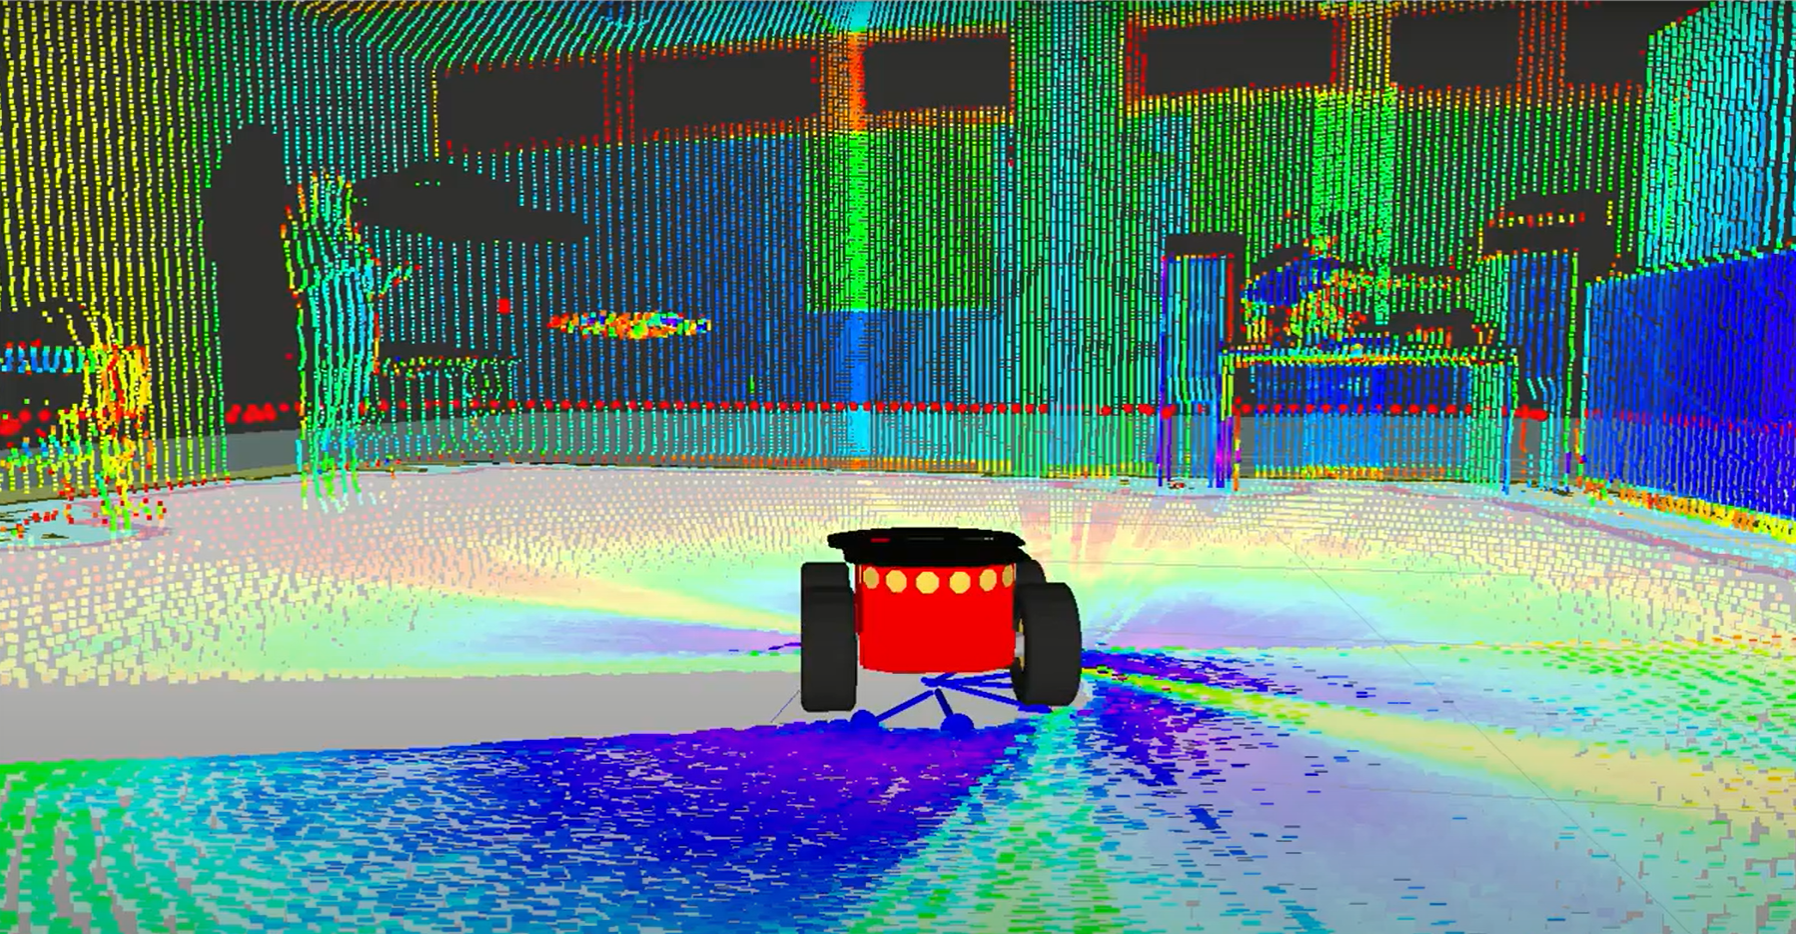
\includegraphics[width=0.5\textwidth]{ch2/figs/lidar_graphic.png}
    \caption{LiDAR scanning and mapping process in mobile robotics.}
    \label{fig:lidar_graphic}
\end{figure}

For this review, two LiDAR sensors will be considered although they will not be considered for the project itself: \textbf{RPLIDAR A1} and \textbf{TF Mini LiDAR (ToF) Laser Range Sensor V2.0}. These sensors offer capabilities that can significantly enhance the robot's ability to perceive and interact with its environment. Below is a comparison of their specifications \cite{yang2022lidar}:

The \textbf{RPLIDAR A1} is a 360-degree scanning LiDAR sensor capable of creating a comprehensive map of the robot's surroundings in real time. This would enable the robot to detect objects and obstacles from all directions, making it ideal for use in complex environments where autonomous navigation is crucial.

\begin{table}[htpb]
\centering
\caption{Comparison of RPLIDAR A1 and TF Mini LiDAR (ToF) Sensors}
\label{tab:lidar_comparison}
\begin{tabular}{|l|l|l|} 
\hline
\textbf{Specification} & \textbf{RPLIDAR A1} & \textbf{TF Mini LiDAR (ToF)}  \\ 
\hline
Max Range              & 12m                 & 12m                           \\ 
\hline
Resolution             & 0.2cm               & 1cm                           \\ 
\hline
Field of View          & 360° (horizontal)   & 3.6° (horizontal)             \\ 
\hline
Sample Rate            & 8000 samples/sec    & 1000 samples/sec              \\ 
\hline
Power Consumption      & 5V, 500mA           & 5V, 140mA                     \\ 
\hline
Interface              & UART, USB           & UART                          \\ 
\hline
Size (mm)              & 97.5 x 60 x 38      & 42 x 15 x 16                  \\
\hline
\end{tabular}
\end{table}

On the other hand, the \textbf{TF Mini LiDAR (ToF)} sensor, although more limited in its field of view, offers a compact and lightweight design, making it suitable for applications requiring focused, high-speed distance measurement. Its small size and low power consumption could be beneficial for tasks where precise distance measurements are needed without adding significant weight or power demands.

Both sensors would improve the robot's environmental mapping and obstacle detection capabilities. Visualizing the LiDAR data in an AR interface would provide real-time feedback to users, enabling them to monitor the robot’s surroundings and make informed decisions about its movement.

\section{Conclusion}

This literature review has explored the integration of Augmented Reality (AR) with mobile robotics, focusing on Human-Robot Interaction (HRI). Key areas such as fiducial marker systems like ArUco markers, sensor technologies, and web-based control interfaces were examined to assess their role in improving real-time visualization and user interaction with robots.

AR has emerged as a crucial tool in enhancing HRI, offering real-time feedback, improved situational awareness, and better task performance. Additionally, sensors such as ultrasonic and LiDAR, combined with AR, hold promise for optimizing navigation and obstacle avoidance in mobile robots.

While AR shows significant potential for advancing HRI, challenges such as real-time processing limitations and the need for secure web-based interfaces remain. These insights will guide the development of my AR framework for the 4WD robotic car, focusing on real-time visualization, intuitive control, and efficient sensor integration.
